\documentclass[titlepage]{econtex}
\immediate\write18{echo akmwwInequality-Discuss > \jobname.bibkey} % Indicate the economics.bib keyname for the entry corresponding to this document

\usepackage{econtexSetup}\usepackage{econtexShortcuts}
\hypersetup{pdfauthor={Christopher D. Carroll <ccarroll@jhu.edu> and Edmund Crawley <edmundcrawley@gmail.com>},
            pdftitle={Discussion of `When Inequality Matters for Macro and Macro Matters for Inequality'}
            pdfcreator = {ccarroll@jhu.edu}
            }
%\DeclareOption{titlepage}{\setcounter{theIncludeTitlePage}{1}}

\begin{document}\large

%\setcounter{theIncludeTitlePage}{0}

\newcommand{\inlinecomment}[2]{\hspace{0in}#2} 

\hfill{\tiny \jobname.tex}

\begin{verbatimwrite}{\jobname.title}
  Discussion of `When Inequality Matters for Macro and Macro Matters for Inequality'
\end{verbatimwrite}


\title{Discussion of \\ `When Inequality Matters for Macro \\ and Macro Matters for Inequality'}

\author{Christopher D. Carroll and Edmund Crawley\num}

\keywords{}

\jelclass{}

\begin{authorsinfo}
\name{Contact: \href{mailto:ccarroll@jhu.edu}{\texttt{ccarroll@jhu.edu}}, Department of Economics, 590 Wyman Hall,
  Johns Hopkins University, Baltimore, MD 21218, \url{http://econ.jhu.edu/people/ccarroll}, and National Bureau of Economic Research.
\href{mailto:edmundcrawley@gmail.com}{\texttt{edmundcrawley@gmail.com}}, Department of Economics, 
Johns Hopkins University, Baltimore, MD 21218.}
\end{authorsinfo}


\maketitleWithForcedDate{July 6, 2017}


\titlepagefinish

\clearpage\vfill\eject
\hypertarget{WhatsWrong}{}
\section{What's Wrong with Macroeconomics, and Can This Paper Fix It?}

For roughly thirty years leading up to the Great Recession, the attention of much of the macroeconomics profession was focused on constructing models in which a single representative agent made optimizing choices that determined the economy's endogenous dynamics.  By a curious (and regrettable) convention, a shorthand term to distinguish such models from their predecessors was to describe them as having ``micro foundations.''

Larry~\cite{summersWolf2} clearly had such models in mind when he summed up his experience at the National Economic Council in the Obama Administration:  ``I would have to say that the vast edifice in both its new Keynesian variety and its new classical variety of attempting to place micro foundations under macroeconomics was not something that informed the policy making process in any important way.''  While Summers's wording was impolite, his view that the new generation of macroeconomic models had little useful to say in the crisis was widely shared among policymakers who were called upon to make difficult decisions at that time.  

After thinking things over, a number of such policymakers including Fed Chair Janet \cite{yellenHetero}, former IMF Chief Economist Olivier \cite{blanchardDSGE}, ECB Governing Board Member Benoit~\cite{coeureHetero}, and Bank of England Chief Economist Andy~\cite{haldaneDappled} have recently suggested that incorporating the right kinds of microeconomic heterogeneity into benchmark macro models would make a major contribution to improving both their performance and their credibility.  

Below, we will suggest that the way to heed this call is to construct models with what we will call `serious' microfoundations (to distinguish them from the models Summers was criticizing, whose claim to be `microfounded' rests on grounds other than matching the pertinent microeconomic evidence).  The paper by AKMWW is an important step in the construction of this new class of models, because the main obstacle to a `seriously' microfounded macroeconomics has long been the mathematical and computational difficulty of solving models with enough heterogeneity (of right kind).  Building on the pioneering work of \cite{reiterSolving,reiterApproximate}, AKMWW describe a methodology and provide a toolkit that promises to vastly expand the scope of questions that can be addressed by models with such heterogeneity.  Providing a toolkit is a key step: Arguably much of the reason for the ubiquity of RA models is the creation of the DYNARE toolkit which vastly simplified construction of such models.\footnote{The first author is PI on a Sloan Foundation grant funding a comprehensive effort to construct a general-purpose toolkit for heterogeneous agent macroeconomics -- and other computational economics topics -- available at \href{econ-ark.org}{http://econ-ark.org}, with the aim of becoming the DYNARE for heterogeneous agents models; incorporation of the AKMWW tools is on the agenda for the \texttt{econ-ark.org} team.}

The paper provides an exhaustive description of its methodological advances, so our discussion will focus on two other questions: Why (and how) serious microfoundations might matter for macroeconomic questions, and the related question of how best to do `quantitative theory' using tools like those the authors provide.\footnote{We endorse  most of the points they make about how macro can matter for inequality, but will leave them undiscussed because this is the NBER Macro Annual and not the NBER Inequality Annual.}
\hypertarget{SeriousHeterogeneity}{}
\section{Why `Serious' Heterogeneity Matters for Macroeconomics}

\subsection{What is `Serious' Heterogeneity?}

A recent paper by~\cite{auclertMPC} distills a key insight from the Heterogeneous Agents (HA) macroeconomics literature:  Auclert produces a reasonably general model with heterogeneous and microconomically optimizing consumers in which, for some questions, the aggregate Marginal Propensity to Consume (MPC -- henceforth, $\bar{\MPC}$) is a `sufficient statistic' for most of what a macroeconomist might need to know about the economy's response to certain kinds of shocks.

One interpretation of Auclert is that the `representative agent' (RA) macroeconomics literature has been handicapped since its origin by the convention that the appropriate target to `represent' is the aggregate wealth-to-income ratio. A standard optimizing consumer with a wealth-to-income ratio of 3 or 4 will inevitably have a value of $\MPC$ closer to 0.03 than to Milton \cite{friedman:windfalls}'s estimate of $\bar{\MPC} \approx 0.33$ (which has held up well in subsequent research -- see below); so to the extent that Auclert's insight generalizes, any model calibrated to match aggregate wealth will badly misrepresent the key `sufficient statistic' required for obtaining the right answer to at least some questions.

Auclert's paper makes it plausible that many macroeconomic questions might be better studied using a `Representative-$\bar{\MPC}$' (for short, `R$\MPC$') model whose single optimizing agent has a target level of wealth at which the MPC matches empirical measures of $\bar{\MPC}$.  (Such models have long been available in the `buffer stock saving' literature (\cite{deatonLiqConstr}; \cite{carroll:bslcpih} explicitly targeted an MPC of 0.4), but were viewed as having little to say about macroeconomics because they made no effort to match aggregate wealth.)

Auclert's paper nevertheless demonstrates that there are many kinds of macroeconomic shocks for which $\bar{\MPC}$ is {\it not} a sufficient statistic -- most prominently (for monetary policy analysis), the effects of interest rate movements.  While it's a good guess that an R$\MPC$ model might do better on many such questions than standard RA models, it would take a long time to rework the bulk of the RA literature as an R$\MPC$ literature; and that reworked literature might uncover deficiencies in the R$\MPC$ model just as serious as those of the RA model.

% Fortunately, we are finally moving beyond the point at which there is a need to designate any single agent as `representative.'

If the HA literature to which AKMWW makes a major methodological contribution succeeds (as we think it ultimately will), workhorse macroeconomic models in the future will dispense altogether with the convenient fiction that the behavior of a single agent can capture everything important about the macroeconomy (whether calibrated to match aggregate wealth or $\bar{\MPC}$).

Of course, households are heterogeneous in an almost unlimited number of ways; in order to be useful, or even feasible, the HA literature will need to make judicious choices about which kinds of heterogeneity are important for macroeconomic analysis, and which can be safely ignored.  The long history of what has worked (and what has not) in the HA literature leads us to the view that a model qualifies as having a `serious' treatment of heterogeneity (by which we mean that it captures the dimensions of heterogeneity that both theory and evidence suggest matter for macroeconomic outcomes) if it:
\begin{enumerate}
\item Matches the microeconomic evidence on the dynamics of household-level income (see motivation below);
\item Produces, as an equilibrium outcome, distributions of wealth and income that match key data on the level and joint distribution of wealth and income, {\it particularly for consumers who the model says should have a high {\MPC}};
\item Generates a $\bar{\MPC}$ that is at least roughly consistent with the vast and diverse microeconomic literature attempting to estimate that object.\footnote{A more ambitious goal would be to match the distribution of $\MPC$ across households; but measuring $\MPC$ at the level of individual households presents such formidable challenges that constructing a population distribution had never even been attempted until national registry data became available very recently; see \cite{fhnMPC} for the first effort we know of.}
\end{enumerate}

The applications of the authors' methodology here, and some previous work by some of them, are among the first examples of models that do a colorable job of satisfying all our criteria of seriousness, and are at the same time capable of being used to simulate and study macroeconomic dynamics.
  The AKMWW paper achieves these goals (at least partially) by following \cite{kvStim} in assuming that even for many wealthy consumers, illiquid assets are largely inaccessible for consumption-smoothing purposes (though the paper makes an important advance over \cite{kvStim} by incorporating empirically calibrated (and large) transitory shocks to income).  

Another, much simpler way to achieve all of these goals is to violate the taboo established by~\cite{bsDigustibus}, and enforced with remarkable rigor in macroeconomics  until recently (though not microeconomics),\footnote{Microeconomists have ignored the injunction; in his Nobel lecture, for example, and a number of other places \cite{HeckmanNobel} has repeatedly argued that measuring and accounting for such heterogeneity is perhaps the central task for microeconomics.} against allowing {\it ex ante} heterogeneity in preferences across consumers.  \cite{ksHetero} broke the taboo, but did not match either $\bar{\MPC}$ or the distribution of wealth.  \cite{cstwMPC} (`CSTW') (and, following them, \cite{kruegerMitmanPerri:handbookMacro}'s chapter in the {\it Handbook of Macroeconomics}) show that all of our proposed elements of `seriousness' can be satisfied by allowing a modest difference in time preference rates (or optimism/pessimism about future growth, or persistent differences in rates of return, or other forms of preference or belief heterogeneity) across consumers, avoiding the complexity associated with modeling the interplay between liquid and illiquid assets. 

\subsection{Implications for Monetary and Fiscal Policy}

While macroeconomists address an enormous range of topics, analysis of most questions partakes strongly of answers to some related question about either monetary or fiscal policy. We will therefore assess the importance of `serious' heterogeneity by asking how its incorporation might change our view of the operation of fiscal and monetary policy, compared to a standard off-the-shelf representative agent New Keynesian (RANK) model of the type that was in 2008, and today still is, widely used at central banks and other policy institutions.  

\subsubsection{Fiscal Policy}

Unless modified to incorporate heterogeneity, such a model would typically imply that a fiscal stimulus payment of the kind implemented by the Bush administration in 2008 (to choose a particularly clean example) would generate extra spending over the subsequent year (an MPC)\footnote{Here and henceforth, quantitative statements about `the MPC' will mean the amount of extra spending that will occur over the next year in consequence of an unanticipated `windfall' shock to income that is not expected to be reversed.}   of only around 0.02 to 0.03 cents on the dollar (even leaving aside the Ricardian Equivalence proposition, which would further attenuate any extra spending).

\cite{brodaParker:stimulus2008}, \cite{psjmMPC2008}, and a number of other papers find estimates of the MPC out of this stimulus payment that are at least an order of magnitude larger than would be implied by a RANK model.  This finding is consistent with a large body of microeconomic evidence spanning the entire interval over which economists have been attempting to estimate the MPC, from \cite{friedmanATheory} to \cite{fhnMPC}, using data of many kinds and from many places and applying to many populations; broadly speaking, estimates of the MPC typically lie somewhere in the range of 0.2 to 0.7.

An illustration of the reason for our earlier proposition that `seriousness' requires matching the wealth distribution {\it particularly for high-$\MPC$ consumers} is captured intuitively in a figure from CSTW, which overlays the empirical distribution of wealth from the U.S. {\it Survey of Consumer Finances} with the consumption functions that characterize the optimal solution to different kinds of consumers' optimal consumption plans.
\begin{figure}
  \caption{Empirical Wealth Distribution and Consumption Functions of Patient and Impatient Agents}
  \label{CFuncDistSevenPointPermAndHistNetWorthPlotFedQuarterly}
\begin{center}
  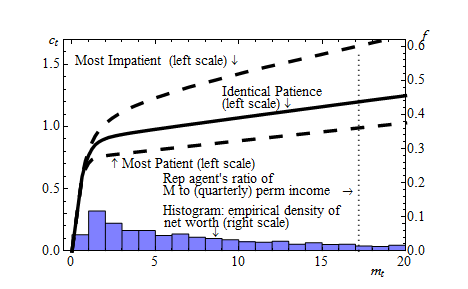
\includegraphics{CFuncDistSevenPointPermAndHistNetWorthPlotFedQuarterly}
\end{center}
\end{figure}
The steeper of the two consumption functions in Figure~\ref{CFuncDistSevenPointPermAndHistNetWorthPlotFedQuarterly} corresponds to the most `impatient' category of consumer in the model; such consumers, in our model's equilibrium, constitute the great majority of the people with low levels of wealth.\footnote{That model matches the data on the wealth distribution at the bottom well, so there is no need to superimpose a third element in the figure.}  The figure shows that the {\it optimal} MPC (that is, the MPC that is the optimal solution of their standard dynamic stochastic optimization problem) is exceptionally high for people with low levels of wealth.

A defender of the current approach to RANK modeling {\it status quo} might object that, with much less work, the high average MPC can be adequately captured by adding to the RANK model some `rule of thumb' consumers {\it a la} \cite{cmModel}'s Macro Annual paper (a `CM model').  This brings us back to Auclert:  His work shows that $\bar{\MPC}$ is a sufficient statistic {\it if that $\bar{\MPC}$ reflects the decisions of optimizing consumers}.  The logic of his argument implies that a model that achieves a high $\bar{\MPC}$ by combining non-optimizing `rule of thumb' consumers with very wealthy `perfect foresight' consumers has no theoretical claim to provide good answers to questions about dynamic macroeconomic questions.

A pertinent illustration of this point comes from a comparison of the implications of the R$\MPC$ and the CM models for the role of uncertainty over the business cycle, which a growing literature suggests is of first order importance.  An optimizing consumer whose $\MPC$ is 0.33 is one whose primary motivation for holding any wealth at all is as a buffer against uncertainty.  When uncertainty rises, that consumer should respond with a sharp cut in spending, in order to build the bigger buffer stock appropriate for the greater degree of uncertainty.  In contrast, the CM `rule of thumb' consumers do not respond at all to uncertainty, and the CM model's wealthy consumers' optimal response would be quite small even if they were to take uncertainty into account in their optimization problem.

\subsubsection{Monetary Policy}

Monetary policy operates via the central bank's control over nominal (and, given the sluggishness of inflation, real) interest rates.  The mechanism by which interest rates affect behavior is therefore the substance of a model's theory of how monetary policy works.

By this standard, RANK models do not have a credible theory of the operation of monetary policy.  Interest rates are hypothesized to affect consumption mainly via the intertemporal substitution channel: When interest rates rise unexpectedly, consumption ought to drop instantly and sharply in response.  The failure of consumption to behave in this manner was recognized in perhaps the first attempt at a structural model of how monetary policy works, by~\cite{rotemberg&woodford:macroannual} in the Macro Annual 20 years ago, and remains a core problem; as ~\cite{blanchardDSGE} has recently put it, ``[The RANK model's] implications with respect to the role of interest rates in twisting the path of consumption, are strongly at odds with the empirical evidence.'' \cite{rotemberg&woodford:macroannual}'s solution was simply to hard-wire a one-year lag into the response of consumption to interest rates, which they invited readers to think of as a crude way to capture the existence of predetermined and unalterable spending plans.  The subsequent literature has adopted subtler expedients, with the most common solution today being the incorporation of habit formation in the utility function of the representative agent.

The habit formation solution has (at least) two problems: There is essentially no microeconomic evidence for the existence of habits (a fact that has held up robustly since \cite{deatonUnderstandingCNotes} articulated it, strongly reinforced by \cite{dynanHabits} and subsequent work); and the introduction of habits substantially further undermines the ability of the model to match the empirical evidence on the MPC.  (Consumers with habits might have an MPC as low as 1 percent).  

Recent work by \cite{kmvHANK} shows that a model with heterogeneous agents provides a major improvement on the benchmark RA model. In a model like the one in AKMWW, but which also includes a New Keynesian production function,  \cite{kmvHANK} find that only about 15 percent of the response of consumption to interest rates is attributable to the (not very credible) intertemporal substitution channel that is essentially the only mechanism for interest rate effects in RANK models.

In sum, `serious' treatment of heterogeneity deeply changes our understanding of the operation of both fiscal and monetary policy, and by implication much of the rest of macroeconomics.  

\section{How to Do Quantitative Theory}

The history of the HA macro literature motivates the `seriousness' criteria we formulated above; different strands of the literature have focused on different elements of seriousness, but (in addition to the computational challenges) part of the reason HA models have been compelling enough to convert the representative macroeconomist to the HA approach is that until recently each previous effort failed in some crucial {\it quantitative} way.

Numerical solutions to models with heterogeneous agents facing uninsurable idiosyncratic risks have been available at least since~\cite{zeldesStochastic}, and efforts to calibrate such models to empirical measurements of household income dynamics have proliferated since the first such effort by~\cite{carroll:brookings}.  The first efforts to construct such a model whose interest rate was consistent with the model-generated aggregate capital-to-output ratio (the most basic definition of a steady-state `general equilibrium') were papers by~\cite{hsz:importance,hsz:insurance}.  \cite{aiyagari:ge} produced a much simpler GE model without a life cycle and with an implausible income process, but which did not require a supercomputer to solve (and thus was much more feasible to build upon).

Aiyagari was focused on the quantitative magnitude of the precautionary saving induced by uninsurable idiosyncratic risks; he found that, when calibrated as he had done, such risks increased the wealth-to-income ratio by only a few percentage points, leading to a natural interpretation that the introduction of idiosyncratic risk made little quantitative difference to macroeconomic outcomes.

These papers failed the `seriousness' criteria above partly because they did not even attempt to match the degree of inequality in the distribution of wealth.  As we now know, many of the quantitative answers obtained from such models (for example, about $\bar{\MPC}$) change drastically when income dynamics and wealth inequality are both matched.  Furthermore, none of these papers could really be used for questions at the heart of macroeconomics involving macroeconomic dynamics.

The first of the major contributions of \cite{ksHetero} was to introduce a method for solving dynamic versions HA models.  But, as in~\cite{aiyagari:ge}, the wealth distribution in the benchmark version of their model was concentrated around the representative agent's wealth, and  the dynamics of their benchmark model differed little from those of a corresponding representative agent model; as a result, many readers reached the conclusion that \cite{ksHetero} had confirmed that heterogeneity did not matter.

That was not the message the authors had intended, and neglected their second major contribution, which was to begin to explore how adding heterogeneity beyond that induced by income shocks might improve the model's fit to the empirical wealth distribution.  While this was a major advance in `seriousness' (as above), even their `dynastic' model greatly understated the degree of wealth inequality; and in particular it produced very few consumers at low levels of wealth where the $\MPC$ is high, and as a result it generated a $\bar{\MPC}$ that was only modestly higher than in the RA model (see \cite{cstwMPC}).  Consequently, even their dynastic model did not have implications profoundly different from those of the corresponding RA model.

The point of this history is that the extent to which heterogeneity matters is a profoundly quantitative question, and answering it credibly turns out to require getting right the quantities that are the key inputs to the model.  This history motivates our `seriousness' criteria above, and leads us back now to discussion of AKMWW.

\subsection{Consumption and Income Dynamics}

\subsubsection{Income Dynamics in Continuous Time}

\cite{friedmanATheory} famously proposed that income has two components: transitory and permanent. A very large subsequent literature, including work with administrative data from the IRS (\cite{dhprvInequality}) and the Social Security Administration (\cite{SabelhausSong}) and work by one of the authors (\cite{kaplanInequality}) has found that Friedman's characterization remains quite a good one, though perhaps the long-lasting shocks that arrive annually are not completely permanent (\cite{dhprvInequality} and \cite{kaplanInequality} estimate the AR(1) coefficient of the persistent component to be 0.97 or 0.98 instead of 1.0).


Being reminded of Friedman's framework helps in thinking through the treatment of income dynamics in AKMWW.  The authors attribute their fantastic increase in computing speed to their use of continuous-time computational tools drawn from the engineering literature.  Unfortunately, there is no neat analogue in continuous time to Friedmanian transitory shocks; the authors argue that their model captures transitory and persistent (nearly permanent) shocks by the Poisson arrival of their $z_1$ and $z_2$ shocks which decay (with perfect predictability, unless another Poisson shock arrives) according to the continuous-time equivalent of an AR(1).  (The authors call this a `jump-drift' process, but because `drift' seems both random and directionless, we will call it a `jump-decay' process).

By matching some moments from~\cite{gkosData}, henceforth GKOS, they calibrate the `transitory' shock $z_1$ to arrive approximately once every 3 years and have a half life of about a quarter, while the `persistent' shock $z_2$ arrives approximately once every 38 years and has a half life of 18 years.

These extreme intervals between shocks (especially the persistent shocks) appear to result from a mismatch between their assumption that income shocks are lognormal, and the enormous kurtosis of annual income shocks estimated by GKOS.

GKOS's describe their own findings as the nail in the coffin of the assumption that income shocks are lognormal.  AKMWW's calibration shows that in principle, it is possible to generate GKOS-sized kurtosis in annual data from a process driven by lognormally distributed jump-decay shocks, but to accomplish that goal it is necessary for the shocks to be very large and very rare.  (A permanent shock that arrives once every 38 years would typically happen at most once in a working lifetime).  In a way, the fact that calibrating lognormal shocks to the GKOS data violates other facts that we know from many other data sources (but that AKMWW do not try to match), is just a confirmation of GKOS's claim that shocks cannot be lognormal.

Another concern is that it is unclear what sort of event the authors' `transitory' shock might represent. The discrete-time equivalent of their continuous-time model would be, for example, to treat the arrival of the 2008 \$600 stimulus checks as though what had actually happened was an increment of roughly \$35 to the consumer's weekly paycheck in the first week, \$33 in the second week, and so on forever (for a sequence whose PDV adds up to \$600). We're certain that Friedman's description of transitory shocks is a much better representation of the 2008 stimulus check than the jump-decay representation, and also feel sure that it is a much better representation of most other transitory movements in income.  Indeed, we have been unable to think of any real-world shocks that resemble their process.

Of course, in principle their solution methods are able to handle any arbitrary calibration of the `transitory' AR(1) process.  If, for example, the specification of the shock were chosen so that, say, 90 percent of the mass of the stimulus payments got paid out in the first week, that would be almost equivalent to a Friedmanian shock.\footnote{The limit of this approach would be a Dirac $\delta$ function that would cause the level of liquid assets to jump discretely; this would result in a Friedman shock, and so presumably at some sufficiently extreme point their computational method would break down.}    Our guess would be that their framework can handle an AR(1) decay that is fast enough to satisfy any reasonable person; but it would be nice to know if that guess is right -- particularly in light of our earlier point that credibility about results in `quantitative theory' models requires credible quantification of the inputs to those models.

In fact, it seems likely that the authors could capture reasonably well a Friedmanian process like that used by most of the prior HA macro literature (including \cite{kaplanInequality}); certainly, they could get a lot closer than they are now to previous models' calibrations, that have been closely tied to the large literature on income dynamics.  Bearing in mind the lesson from the history of the HA literature that calibrational assumptions matter profoundly for quantitative conclusions, some caution is warranted in the interpretation of all of their quantitative results.

\subsubsection{What is `the MPC' Out of A Transitory Shock?}

Another concern about the authors' calibration is that the right way to compute something that can be designated as `the MPC' out of one of their $z_{1}$ `transitory' shocks is not so obvious.

Since, in continuous time, both income and consumption are flow variables, only when the flow has been integrated over some finite interval does it become possible to speak of a `marginal propensity to consume' -- over that interval.  Hence our explicit earlier definition above of $\MPC$ as the amount of extra spending {\it over the subsequent year} induced by the arrival of a transitory shock.  Concretely, then, `the MPC' over one period (between $t$ and $t+1$) out of a lump sum Friedmanian transitory shock of size \$x at date $t$ would be
\begin{eqnarray}
  \MPC & = & \frac{\int_{t}^{t+1} (c_{\tau}-c^{*}_\tau)~ d\tau}{x}
\end{eqnarray}
where $c^{*}_\tau$ is the consumption that would have occurred in the absence of the shock.

Indeed this is the method used for calculating what the authors report as `the MPC' in the paper, despite the fact that Friedmanian shocks are not what is expected by the consumers in the model.  (Thus their MPC is calculated as the consequence of what has recently come to be referred to as `an MIT shock').  

If the authors wanted to calculate the `MPC out of a transitory shock' for the model-consistent transitory shocks that their consumers experience, the numerator would be the same as in the equation above, but they would have have (at least) two choices for the denominator.  The first would be to integrate the flow of transitory income over the same interval that applies to consumption:
\begin{eqnarray}
  x_{a} & = & \int_{t}^{t+1} z_{1,\tau} d \tau.
\end{eqnarray}
The other is to use the entire PDV of the shock as the denominator,
\begin{eqnarray}
  x_{b} & =& \int_{t}^{\infty} z_{1,\tau} d\tau
\end{eqnarray}

If virtually all of the transitory shock has arrived by the beginning of period $t+1$, the two measures will be almost the same.  But at the quarterly frequency, their transitory shock's flow has only fallen by half, so there is a great deal more income that has yet to reach the consumer.  

So, unless the AR(1) coefficient is quite small (and theirs is not), there can be a substantial difference between the MPC out of a Friedman transitory shock and the MPC out of their transitory shock.

What we're less sure of is how much the discrepancy matters; there are circumstances under which their shock would have effects virtually identical to those the Friedman shock.  In the certainty-equivalent (CEQ) or the perfect foresight (PF) formulations of the permanent income hypothesis, consumption is a function of the PDV of income, without regard to income's timing.  But, what this means is that the circumstances in which their shock is equivalent to a Friedman shock are basically the circumstances under which their model most closely resembles the CEQ/PF model.  Thus, to some degree, the more different their model is from the CEQ/PF model, the less plausible is their treatment of transitory shocks, and the only way to get around this tradeoff is to make the AR(1) decay speed very rapid.


\subsubsection{Excess Sensitivity and Excess Smoothness}

The authors use their two-asset model to see how well it can match the empirical phenomena of excess sensitivity and excess smoothness. 


It is not clear that the results from the two-asset model are an overall improvement on existing models (see table 9); the most striking result is their model's Campbell-Mankiw coefficient of 0.98. This contrasts with essentially 0.00 for the representative agent model and 0.49 in the data. The authors account for this large coefficient by the existence of hand-to-mouth consumers who do not smooth their consumption over time. However, the quarterly MPC in their model is 22 percent. A naive estimate of the Campbell-Mankiw coefficient in their model might then be 0.22 in a similar way that the saver-spender model with 50 percent hand-to-mouth consumers leads to a Campbell-Mankiw coefficient of 0.5. Exactly why this is not so is worthy of further investigation. We believe that the coefficient may be very sensitive to two unconventional ways in which the model is calibrated.

First, they model income \textit{growth} as an AR(1).  \cite{cdSmooth} pointed out long ago that if income \textit{growth} follows an AR(1), then permanent income goes up more than one-to-one with an unexpected increase in income, and therefore in a CEQ model, consumption would be expected to increase by more than the change in current income. Unfortunately, our short macro time-series are not very informative about the nature of the income process, particularly in the long run (see \cite{stock_confidence_1991}). The ratio of the volatility of consumption to the volatility of income (another statistic reported in the paper) should be highly sensitive to the exact assumption about the income growth process and we suspect the Campbell-Mankiw coefficient is likely to be similarly sensitive; so we are doubtful that their 0.98 Campbell-Mankiw coefficient would be robust to alternative choices of income growth processes.

Second, in order to make comparison with the one-asset models more straightforward, the authors assume that the supply of the liquid asset is elastic. Implicitly, it is is as though the liquid asset freely trades as in a small open economy, but there are strict capital controls on the illiquid asset. We have not succeed in thinking this through completely,  but are concerned that this may open up large differences between the two interest rates upon arrival of a positive TFP shock. In turn, that might result in many more consumers hitting their borrowing constraint in order to invest at the higher interest rate available in the illiquid asset. A bit more investigation into the exact mechanism here, along with some empirical work as to whether it is reasonable, would help us understand whether the high Campbell-Mankiw coefficient in the model should be taken seriously.


\subsection{A Note on the Failure of Approximate Aggregation}
The computational methods presented in the paper are particularly applicable for models where `approximate aggregation' (per Krusell and Smith) fails. This is important to their model's solution, because the failure of approximate aggregation in the authors' two-asset model is extreme. While the Krusell-Smith algorithm needs just one state variable to retrieve the path of wages and interest rates to a very high degree of accuracy, the authors find that 300 or more dimensions are required for their two asset model.

Of course, for showing off their toolkit's powers, a model that is not easily represented by a small basis is ideal.  But as economists we would like to understand what is driving the dynamics of our models. The high dimensionality of the two-asset model implies that small changes in particular parts of the distribution can significantly alter the path of prices, particularly of the liquid asset; it would be a formidable challenge to obtain some intuition for the mechanisms involved.  A related problem is that, if even economists have trouble understanding the mechanics of the model, the assumption that all consumers understand it perfectly (as required by their rational expectations solution method) is far more questionable than when the economy's dynamics are relatively simple.

A possible resolution of this puzzle is that the basis that the authors make available to their algorithm is inefficient. The motivation for the basis comes from matching the first k terms of the Taylor series for the impulse response of prices around the time of impact (see equations 30 and 31). For an exogenous decision rule the basis is chosen to be an exact match. For endogenous decisions rules (such as those in economic models), the basis is chosen by ignoring the feedback from individuals' decisions to the distribution. While this means the terms of the Taylor series are no longer exactly matched, the hope is that the assumption may be approximately true and the resulting basis will nevertheless allow for a large reduction in dimension. Figure 7 shows the impulse response for different orders of distribution reduction. If the first k terms of the Taylor expansion were well approximated, we would expect that the impulse response would be accurate for small values of t, deteriorating as the time from impact increases. This is indeed the case for the illiquid return and wage impulse responses. The k=2 approximation to the impulse response for the liquid asset, on the other hand, is most inaccurate for small values of t. This suggests the failure of approximate aggregation may be as much due to having chosen an inefficient basis as to the underlying economic structure.

The authors suggest an iterative procedure to improve the efficiency of the basis in cases where the degree of dimension reduction in the basic algorithm is still not enough to make the model numerically tractable. It should be possible to use the same algorithm to find an efficient basis that accurately matches the first k terms of the impulse response Taylor expansion. Replicating figure 7 with this new basis should match the liquid return well for small values of t and it would be interesting to know how well it does for larger values of t. It is our guess that finding a better basis would not only improve the computational performance of their algorithm, but also might shed light on the economic forces driving the model.

\section{Conclusion}

This paper comes at a good time.  A critical mass of policymakers and academics seems to have been convinced by the events of the Great Recession that the incorporation of `serious' heterogeneity will be essential to the creation of a new generation of macroeconomic models that will be more useful than existing benchmark models (and more credible, because of their correspondence with microeconomic evidence).  And, prior work in the HA literature has converged on something like a consensus about the kinds of heterogeneity that will be needed.  

This paper offers tools that promise to help remove the chief barrier to the construction of such models, which is the computational bottleneck that has profoundly restricted the extent to which models including serious heterogeneity could be used to perform general purpose macroeconomic analysis.  As with any new tool, the immediate agenda is to confirm that the tool works for problems whose solution is well known, to build a bridge between what is known now and what will be possible in the future.  The authors have done that already with the canonical Krusell-Smith model, and we are confident that, with some adjustment to its calibration choices, it will be possible to show that the model can be used to obtain essentially the same results that other papers in the existing literature have obtained, but several orders of magnitude faster.  Once that is done, the floodgates will be open for a new generation of general purpose macro models that will truly deserve to be called `microfounded.'

\normalsize

\input econtexBibMake

\end{document}

